\documentclass[letterpaper,10pt]{article}

\usepackage{enumitem}
\usepackage{titling}
\usepackage{listings,listings-rust}
\usepackage{url}
\usepackage{soul}
\usepackage{hyperref}
\usepackage{setspace}
\usepackage{subfig}
\usepackage{sectsty}
\usepackage{pdfpages}
\usepackage{colortbl}
\usepackage{multirow}
\usepackage{multicol}
\usepackage{relsize}
\usepackage{amsmath}
\usepackage{wasysym}
\usepackage{fancyvrb}
\usepackage[yyyymmdd]{datetime}
\usepackage{amsmath,amssymb,amsthm,graphicx,xspace}
\usepackage[titlenotnumbered,noend,noline]{algorithm2e}
\usepackage[compact]{titlesec}
\usepackage{XCharter}
\usepackage[T1]{fontenc}
\usepackage[scaled]{beramono}
\usepackage[normalem]{ulem}
\usepackage{booktabs}
\usepackage{tikz}
\usetikzlibrary{arrows.meta,automata,shapes,trees,matrix,chains,scopes,positioning,calc,decorations.pathreplacing}
\tikzstyle{block} = [rectangle, draw, fill=blue!20, 
    text width=2.5em, text centered, rounded corners, minimum height=2em]
\tikzstyle{bw} = [rectangle, draw, fill=blue!20, 
    text width=4em, text centered, rounded corners, minimum height=2em]

\definecolor{namerow}{cmyk}{.40,.40,.40,.40}
\definecolor{namecol}{cmyk}{.40,.40,.40,.40}
\renewcommand{\dateseparator}{-}

\let\LaTeXtitle\title
\renewcommand{\title}[1]{\LaTeXtitle{\textsf{#1}}}

\lstset{basicstyle=\footnotesize\ttfamily,breaklines=true}

\newcommand{\CPP}{C\nolinebreak\hspace{-.05em}\raisebox{.4ex}{\tiny\bf +}\nolinebreak\hspace{-.10em}\raisebox{.4ex}{\tiny\bf +}}
\def\CPP{{C\nolinebreak[4]\hspace{-.05em}\raisebox{.4ex}{\tiny\bf ++}}}

\newcommand{\handout}[5]{
  \noindent
  \begin{center}
  \framebox{
    \vbox{
      \hbox to 5.78in { {\bf ECE459: Programming for Performance } \hfill #2 }
      \vspace{4mm}
      \hbox to 5.78in { {\Large \hfill #4  \hfill} }
      \vspace{2mm}
      \hbox to 5.78in { {\em #3 \hfill \today} }
    }
  }
  \end{center}
  \vspace*{4mm}
}

\newcommand{\lecture}[3]{\handout{#1}{#2}{#3}{Lecture#1}}
\newcommand{\tuple}[1]{\ensuremath{\left\langle #1 \right\rangle}\xspace}

\addtolength{\oddsidemargin}{-1.000in}
\addtolength{\evensidemargin}{-0.500in}
\addtolength{\textwidth}{2.0in}
\addtolength{\topmargin}{-1.000in}
\addtolength{\textheight}{1.75in}
\addtolength{\parskip}{\baselineskip}
\setlength{\parindent}{0in}
\renewcommand{\baselinestretch}{1.5}
\newcommand{\term}{Winter 2020}

\singlespace


\begin{document}

\lecture{ 3 --- Rust: Borrowing, Slices }{\term}{Jeff Zarnett}

\section*{Borrowing and References}
We've already seen that ownership is a concept in Rust that can come with a couple of unintended consequences, like accidentally giving an argument to a function that we still need later. Rust allows us the idea of ``borrowing'' -- you need to use the data for something but you also promise you'll give it back. It allows data to be shared, but the sharing has to be done in a controlled and safe way to prevent the possibility of race conditions.

Rust's compiler analyzes all the borrowing that takes place in the program using the \textit{borrow checker}. If the borrow checker is not certain that your code is perfectly safe, it will say no (and produce a compile time error). This can be a little bit frustrating, because the analysis is not perfect and errs on the side of caution. Eventually we will introduce some ways that you can tell the borrow checker that you guarantee the code is safe, but you have to be sure, otherwise all the usual bad things can happen!

The feature that we need for the concept of borrowing is the \textit{reference}. To indicate that you want to use a reference, use the \texttt{\&} operator. The reference operator is appears both on the function definition and the invocation, to make sure there's no possibility of confusion as to whether a reference is being expected/provided or ownership is to be transferred.  Consider this example from the official docs~\cite{rustdocs}:

\begin{lstlisting}[language=Rust]
fn main() {
    let s1 = String::from("hello");
    let len = calculate_length(&s1);
    println!("The length of '{}' is {}.", s1, len);
}

fn calculate_length(s: &String) -> usize {
    s.len()
}
\end{lstlisting}

So when we invoke the \texttt{calculate\_length} function, ownership of the string is not transferred, but instead a reference to it is provided. The reference goes out of scope at the end of the function where it was used, removing it from consideration. A reference is not the same as ownership and the reference cannot exist without the original owner continuing to exist. That is represented in the official docs by this diagram:

\begin{center}
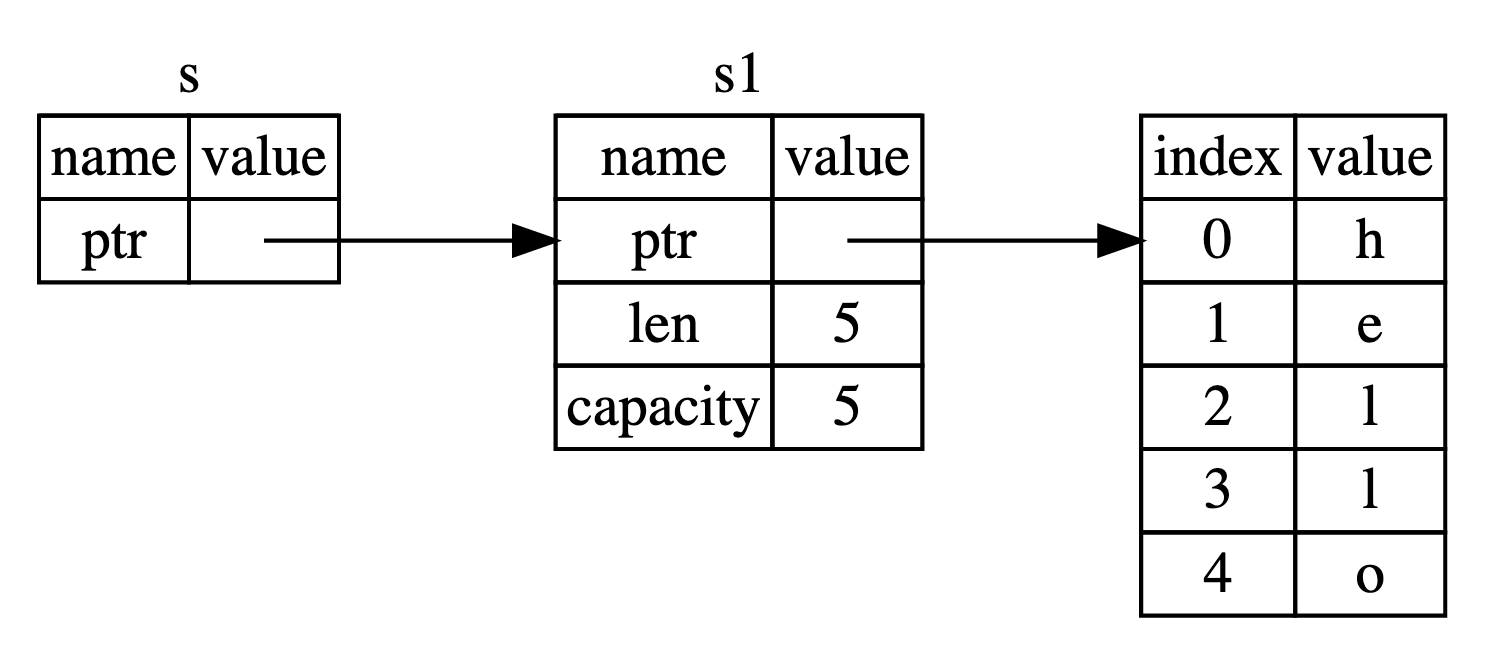
\includegraphics[width=0.5\textwidth]{images/string-with-ref.png}
\end{center}

And if you borrow something, it's not yours to do with as you wish -- you cannot assign ownership of it (move it), which makes sense because you can't give someone ownership of something you do not own.

By default, references are immutable: if you borrow something, you cannot change it, even if the underlying data is mutable. Attempting to do so will result in -- you guessed it -- a compile time error, where the compiler tells you that you are trying to change something that's immutable. 

Of course, in real life, you would be much more agreeable to letting people borrow your things if there were strong guarantees that it would (1) always be returned and (2) would be returned in the same condition. That would be nice! But until such time as that magical technology is invented, no, you can't borrow my car. Sorry.

Mutable references do exist, but they have to be declared explicitly as such by tagging them as \texttt{\&mut}:

\begin{lstlisting}
fn main() {
    let s1 = String::from("hello");
    let len = calculate_length(&mut s1);
    println!("The length of '{}' is {}.", s1, len);
}

fn calculate_length(s: &mut String) -> usize {
    s.len()
}
\end{lstlisting}

Mutable references come with  some big restrictions: (1) while a mutable reference exists, the owner can't change the data, and (2) there can be only one mutable reference at a time, and when there is, there can be no immutable references. This is, once again, to prevent the possibility of a race condition. These two restrictions ensure that there aren't concurrent accesses to the data when writes are possible. There's also a potential performance increase where values can be cached (including in CPU registers; we'll come to that later) without worry that they will get out of date.

As long as there are no mutable references, there can be arbitrarily many immutable references at the same time, because reads don't interfere with reads and a race condition does not occur if there are only reads. 

References cannot outlive their underlying objects. Below is an example from the official docs that will be rejected by the borrow checker, because the reference returned in \texttt{dangle} refers to memory whose owner \texttt{s} goes out of scope at the end of the function:

\begin{lstlisting}[language=Rust]
fn main() {
    let reference_to_nothing = dangle();
}

fn dangle() -> &String {
    let s = String::from("hello");
    &s
}
\end{lstlisting} 

In C this would be a ``dangling pointer'' (a pointer that's pointing to a location that is no longer valid). I see this kind of error a lot in C programs where someone has stack allocated a structure and then wants to pass it to another thread and does so with the address-of operator. It compiles and might even work sometimes at runtime, but is still wrong and can eventually lead to a bug that bites you. 

If we actually try to compile the previous code example, the compiler says something about giving the value a lifetime. We'll come back to the idea of lifetimes soon.

\paragraph{Non-Lexical Lifetimes.} A more recent improvement to Rust's borrow checking is called non-Lexical lifetimes. Consider the small block of code below:
\begin{lstlisting}[language=Rust]
fn main() {
    let mut x = 5;

    let y = &x;
    println!("{}", y);

    let z = &mut x;
}
\end{lstlisting}

Under the old rules, the compiler would not allow creation of the mutable reference \texttt{z} because \texttt{y} has not gone out of scope. It would consider \texttt{y} to be valid until the end of the function. The improvement of NLL is that the compiler can see that \texttt{y} is no longer used after the \texttt{println!} macro and the \texttt{z} reference is okay to create. The compiler will then make it so that \texttt{y} is removed as soon as it's no longer needed so the \texttt{z} reference will not exist at the same time and all is fine.

\subsection*{Slices}
The \textit{slice} concept exists in a few other programming languages, and if you have experience with them this will certainly help. A slice is a reference (yes, a reference in the sense of the previous section) to a contiguous subset of the elements of a collection. This is what you do if you need a part of an array (the typical example for that being a substring of an existing string). If our code looks like this:

\begin{lstlisting}[language=Rust]
fn main() {
    let s = String::from("hello world");
    let hello = &s[0..5];
    let world = &s[6..11];
}
\end{lstlisting}

The representation of the slice looks like~\cite{rustdocs}:
\begin{center}
	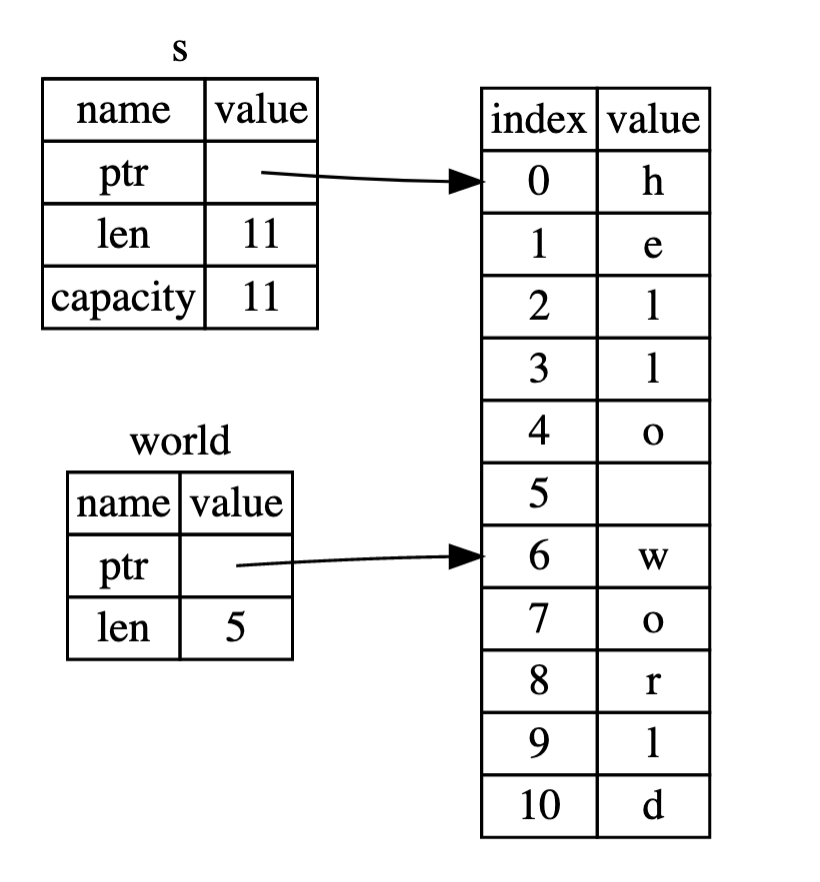
\includegraphics[width=0.3\textwidth]{images/string-slice.png}
\end{center}

Slices can also apply to vectors and other collections; not just strings. As with the other kinds of references we've learned about, the existence of a slice prevents modification of the underlying data. Just as with references, slices prevent race conditions on collections but also avoid (as much as possible) the need to copy data (slow).

\bibliographystyle{alphaurl}
\bibliography{459}


\end{document}
